\section{Data}
\label{sec:data}

\subsection{Dataset, Preselection and Mass}
\label{sec:data_presel}
\emph{In short: $8{,}556{,}118$ candidates are reduced to $23{,}895$ by a kaon-identification and muon-veto requirement common to the analyses; the fit window $[5100,5600]\,\MeV$ contains $19{,}731$ candidates ($10{,}292$ $B^+$, $9439$ $B^-$).}
The dataset is the CERN Open Data record 4900~\cite{opendata_record}: $B^{\pm}\to h^{\pm}h^{+}h^{-}$ candidates collected by LHCb in 2011 at $\sqrt{s}=7$\,TeV, already through trigger and offline selection, distributed as ROOT \texttt{TTree}s with the most relevant branches and split by magnet polarity, for $8{,}556{,}118$ candidates. The record also contains a phase-space simulation of $B^{\pm}\to K^{\pm}K^{+}K^{-}$ ($50{,}000$ decays, no asymmetry), used only to test the local-asymmetry procedure (Sec.~\ref{sec:dalitz}).

\begin{table}[h]
\centering
\resizebox{\ifdim\width>\linewidth\linewidth\else\width\fi}{!}{\begin{tabular}{lrrrr}
\toprule
Requirement & alone & cumulative & down & up \\
\midrule
All candidates & -- & $8{,}556{,}118$ & $5{,}135{,}823$ & $3{,}420{,}295$ \\
$\lnot\texttt{isMuon}$, three tracks & $6{,}311{,}517$ & $6{,}311{,}517$ & $3{,}806{,}297$ & $2{,}505{,}220$ \\
$\texttt{ProbPi}<0.5$, three tracks & $975{,}724$ & $481{,}101$ & $288{,}908$ & $192{,}193$ \\
$\texttt{ProbK}>0.5$, three tracks & $28{,}812$ & $23{,}895$ & $14{,}178$ & $9717$ \\
Mass window $[5100,5600]\,\MeV$ & -- & $19{,}731$ & $11{,}636$ & $8095$ \\
\bottomrule
\end{tabular}}
\caption{Number of candidates passing each requirement alone and after the cumulative selection, in the order of the table, and by magnet polarity. The kaon-identification requirement on the three tracks is by far the most selective.}
\label{tab:cutflow}
\end{table}

For each of the three final-state tracks ($H1$, $H2$, $H3$) the analysis reads the momentum components, the particle-identification (PID) likelihoods (\texttt{ProbK}, \texttt{ProbPi}), a muon flag and the charge. The same preselection is used in all analyses,
\[
\texttt{H*\_ProbPi} < 0.5 \ \wedge\ \texttt{H*\_ProbK} > 0.5 \ \wedge\ \lnot\texttt{H*\_isMuon},
\]
and retains $23{,}895$ of the $8{,}556{,}118$ candidates ($0.28\%$), the PID requirement being the dominant reduction (Table~\ref{tab:cutflow}).

$H1$ is always the kaon of charge opposite to the $B$ and $H2$, $H3$ the interchangeable same-sign pair, so the Dalitz variables are $m^2(H1,H2)$ and $m^2(H1,H3)$.

\label{sec:data_mass}
The three final-state tracks are assigned the charged-kaon mass hypothesis ($M_K=493.677\,\MeV$) regardless of their PID likelihoods, and their four-momenta are summed to reconstruct the $B$ candidate, $m(KKK)=\sqrt{(\sum_i E_i)^2-|\sum_i \vec{p}_i|^2}$. The nominal fit window, common to the frequentist and Bayesian analyses, is $[5100,5600]\,\MeV$ and contains $19{,}731$ candidates ($10{,}292$ $B^+$, $9439$ $B^-$; $11{,}636$ magnet down, $8095$ magnet up). Below $\sim$5150\,\MeV\ the background rises, consistent with a partially reconstructed contribution that a single exponential cannot describe; the window includes the start of this rise, which is described by a second exponential in the background model (Secs.~\ref{sec:frequentist}--\ref{sec:bayesian}). The machine-learning selection (Appendix~\ref{sec:ml}) uses the same window.

\subsection{Data Exploration}
\label{sec:data_exploration}
\emph{In short: the spectrum peaks at $5284\,\MeV$ with a similar shape for the two charges and the two magnet polarities, and the counting asymmetry of all candidates is $-0.043\pm0.007$.}
\begin{figure*}[t]
\centering
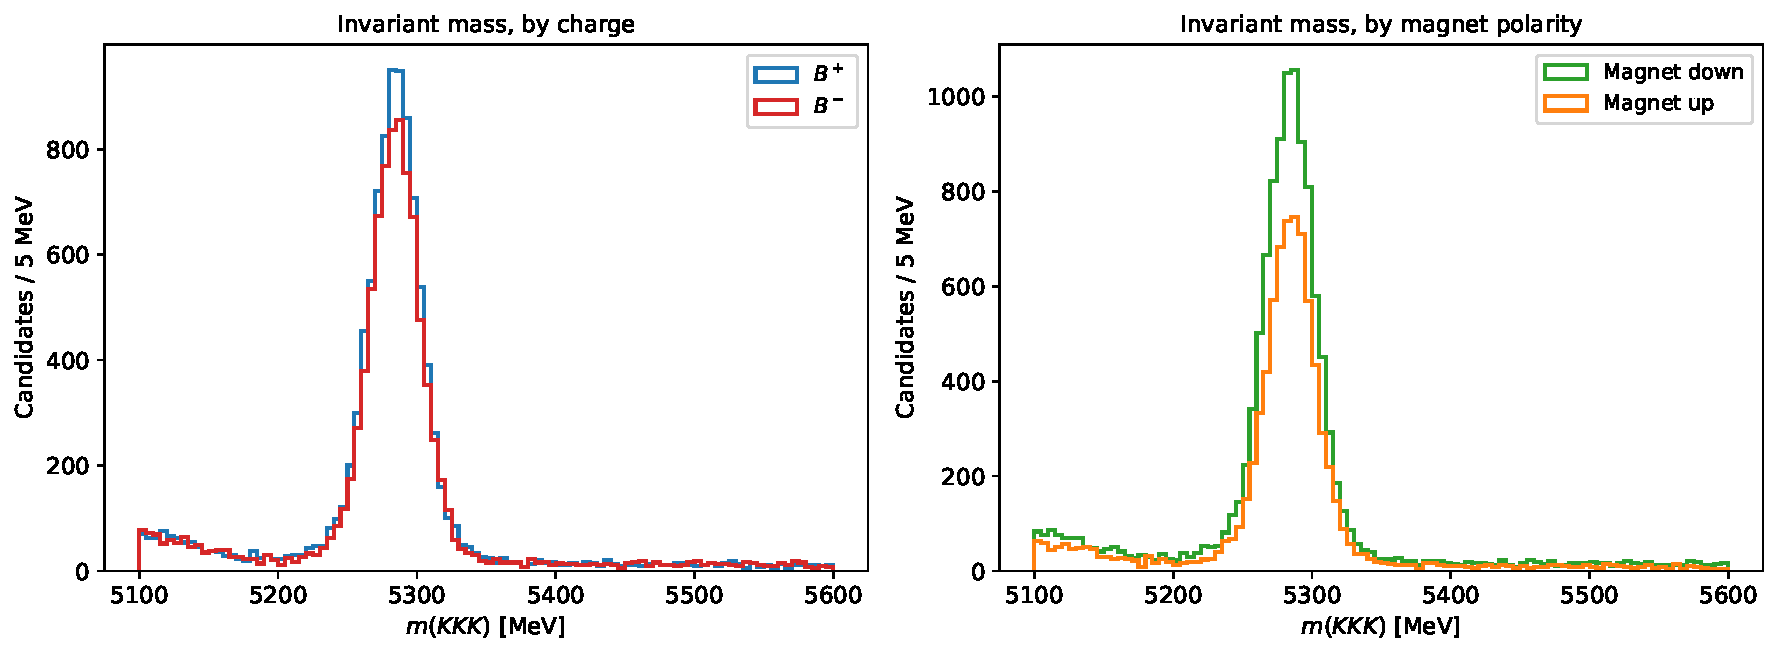
\includegraphics[width=0.95\textwidth]{figures/mass_spectrum.pdf}
\caption{Reconstructed $B\to KKK$ invariant mass in the nominal fit window $[5100,5600]\,\MeV$, split by (a) $B$ charge and (b) magnet polarity. Both splits show a consistent peak at $m\approx5284\,\MeV$ over a falling combinatorial background, which rises below $\sim$5150\,\MeV.}
\label{fig:mass_spectrum}
\end{figure*}

Figure~\ref{fig:mass_spectrum} shows the reconstructed mass spectrum in the fit window, split by $B$ charge (left) and by magnet polarity (right). The spectrum peaks at $m\approx5284\,\MeV$ over a falling combinatorial background, with a similar shape for the two charges and the two magnet polarities. The charge-counting asymmetry of all candidates in the fit window, signal and background together, is $A_{\mathrm{count}}=(N^--N^+)/(N^-+N^+)=-0.043\pm0.007$ (binomial uncertainty).


